

% Chapter 1

\chapter{Robot} % Main chapter title

\label{Chapter2} % For referencing the chapter elsewhere, use \ref{Chapter1} 

\lhead{Capítulo 2. \emph{Robot}} % This is for the header on each page - perhaps a shortened title

%----------------------------------------------------------------------------------------

%--------------------------------------------------------
%Sección 1
%--------------------------------------------------------

\begin{figure}[htbp]
	\centering
		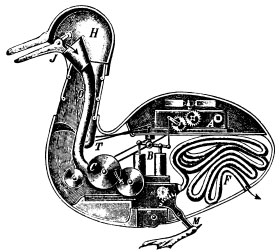
\includegraphics[width=0.6\textwidth]{./Figures/Duck_of_Vaucanson.jpg}
		\rule{35em}{0.5pt}
	\caption[Robot Digesting Duck]{Digesting Duck, creado por Jacques de Vaucanson en 1739. Imagen tomada de Wikipedia.}
	\label{fig:Duck}
\end{figure}



\section{¿Qué es un robot?}

Un robot puede ser un software solamente o tener además una extensión física que le permita desempeñar tareas realizadas por el ser humano o que necesitan algo de inteligencia. El término robot se le atribuye al dramaturgo checo Karel Čapek, que en su obra R.U.R en 1921 (Rossum’s Universal Robots) utilizó la palabra \textit{robotnik} para referirse a ayudantes artificiales. Luego fue el escritor Isaac Asimov (1920-1992) quien,  gracias a su obra, difundió la palabra robótica haciendo referencia a la ciencia encargada de estudiar a los robots. Él desarrolló las Tres Leyes de la Robótica, que son una especia de normativa que regula el comportamiento de los robot en sus libros de Ciencia Ficción. La robótica como ciencia contempla el estudio de al menos 6 áreas: La mecánica, la electrónica, la informática, el control automático, la física y la matemática.

En la historia hay varios intentos por construir estos ayudantes artificiales. A principios del siglo XVIII, Jacques de Vaucanson creó un autómata capaz de tocar la flauta, así como un pato mecánico que continuamente seguía su ciclo biológico, ver figura \ref{fig:Duck}.

En la actualidad las empresas KUKA, Honda y Sony, entre otras, construyen robots especialmente diseñados para la industria. Los robots que se utilizan en la industria, y los pocos que han llegado al hogar, son controlados por un algoritmo. Este es parte de un software que escribe una persona, donde se detalla la tarea que el robot debe realizar; tiene un modelo de los motores, partes y piezas para que así la máquina tenga información de como es, y pueda ejecutar la tarea para la cual se le programó. Si se interfiere con el entorno del robot, por ejemplo moviendo 1 [cm], fuera del rango de los sensores, el perno que debe apretar algún robot industrial que ensambla autos, este no podrá \textit{encontrarlo}. No todos los robots comerciales que existen hoy en día son capaces de adaptarse a cambios en el entorno (hay algunos que poseen sistemas de visión que permiten hacer estas correcciones) y menos ser capaces de generar una imagen de sí mismos que les permita entender qué sucede y recuperarse de fallas.

\begin{figure}[htbp]
	\centering
		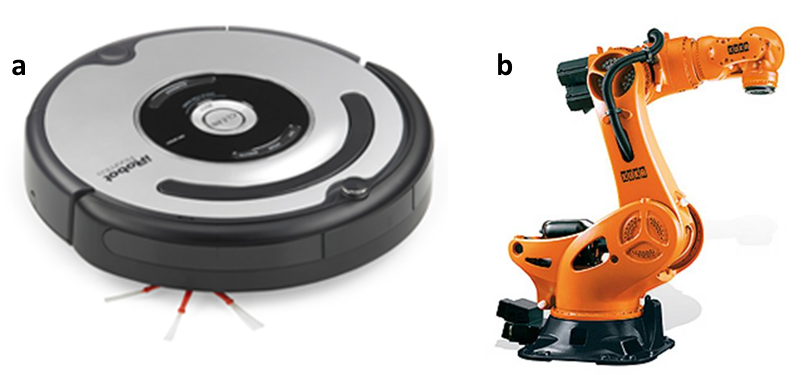
\includegraphics[width=\textwidth]{./Figures/RobotsInd.png}
		\rule{35em}{0.5pt}
	\caption[Robots Roomba y KUKA]{\textbf{a. }Robot Roomba, primer Robot domestico vendido en chile. Imagen tomada de \cite{Forlizzi:2006:SRD:1121241.1121286} \textbf{b.} Robot industrial KUKA KR 1000 TITAM. Imagen tomada de kuka-robotics.com}
	\label{fig:Roomba y KUKA}
\end{figure}

Para programar el software de control en un robot, se debe tener un modelo detallado de los motores y sensores que se poseen y es tarea del programador hacer la abstracción necesaria para poder darle sentido al movimiento del conjunto de motores. Cada motor aporta con un grado de libertad,o por su sigla en ingles DOF (degree of freedom). Los Grados de libertad hacen referencia al número de movimientos independientes que se pueden realizar. En otras palabras, un grado de libertad es la capacidad de moverse a lo largo de un eje (movimiento lineal) o de rotar a largo de un eje (movimiento rotacional). Por ejemplo, un auto posee 3 grados de libertad, dos de posición y uno de orientación. 

Si hablamos de un robot de 4 extremidades, con 3 grados de libertad en cada una, el programador debe ser capaz de indicar la secuencia de activación de cada motor. Primero debe hacer que el robot mueva una extremidad y luego con la suma de las 4 lograr desplazarse. Estamos hablando de 12 motores que pueden moverse de forma independiente,lo cual genera infinitas soluciones y no todas posibles debido a las restricciones físicas de la construcción misma del robot.

\begin{figure}[htbp]
	\centering
		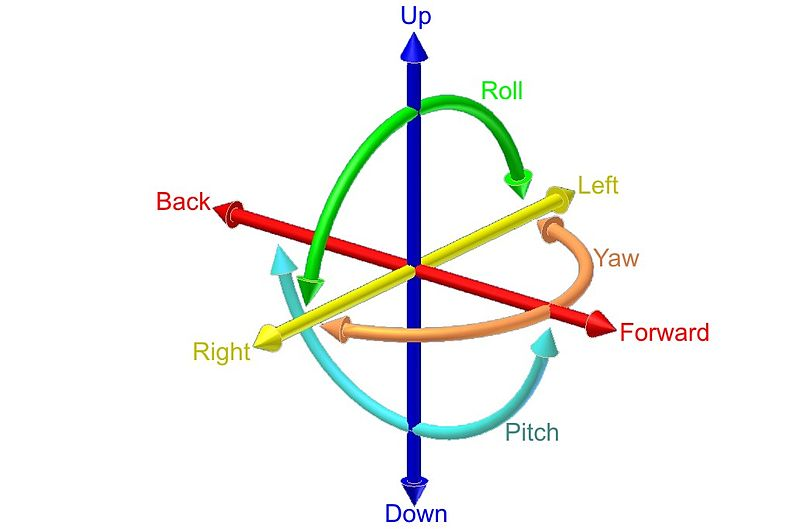
\includegraphics[width=\textwidth]{./Figures/6DOF.jpg}
		\rule{35em}{0.5pt}
	\caption[Grados de libertad]{Seis grados de libertad, tres son de desplazamiento y tres son de orientación. Imagen tomada de Wikipedia.}
	\label{fig:grados de libertad}
\end{figure}



